% appendix.tex -- de (German)
Der Anhang enth�lt die EAGLE-Zeichnungen zur TinkerKit-Zusatzplatine:
\begin{compactitem}
	\item Verdrahtungskonzept der TinkerKit-Taster
	\item Schaltplan der TinkerKit-Zusatzplatine
	\item Leiterplatte
	\begin{compactitem}
		\item Abmessungen
		\item Oberseite
		\item Unterseite
	\end{compactitem}
%	\item Best�ckung
\end{compactitem}

\section{Best�ckvarianten}
Die Leiterplatte kann so best�ckt werden, dass sie funktional dem in
Abschnitt \ref{sect:TinkerKitBoard} beschriebenen Prototypen
entspricht.\\
Alternativ kann die Best�ckung f�r sechs �ber Spannungsteiler
unterscheidbare Taster an den analogen Eing�ngen der wei�en 
TinkerKit-Anschl�sse ausgef�hrt werden. Die Taster f�r die digitalen
TinkerKit-Anschl�sse (orange) k�nnen an anderer Stelle (\zB als
Schultertasten am Geh�use) verbaut werden und an der Stiftleiste X1
angeschlossen werden.

Die gew�nschte Version kann �ber die dazugeh�rige Best�ckvariante aus
Tabelle \ref{tab:variants} festgelegt werden:

\begin{table}[h]
\centering
\renewcommand{\arraystretch}{1.5}
\begin{tabular}{|p{0.23\textwidth}|p{0.16\textwidth}|p{0.18\textwidth}|p{0.15\textwidth}|p{0.16\textwidth}|}
\hline
\textbf{Version}								&	\textbf{RDIG\_ORL, RDIG\_ORR}	&	\textbf{RANA\_ORL, RANA\_ORR}	&	\textbf{RDN\_ORL, RDN\_ORR}	&	\textbf{RDN\_PINL, RDN\_PINR}\\
\hline
	vier analoge Taster,\newline zwei digitale Taster	&	0R								&	nicht best�ckt					&	1k							&	nicht best�ckt\\
\hline
	sechs analoge Taster,\newline zwei externe Taster	&	nicht best�ckt					&	0R								&	68k oder 82k (t.b.d.)		&	1k\\
\hline
\end{tabular}
\vspace{0.5cm}
\caption{Best�ckvarianten}
\label{tab:variants}
\end{table}




%---------------------------------------------------------------
%  conception
%---------------------------------------------------------------
%%%%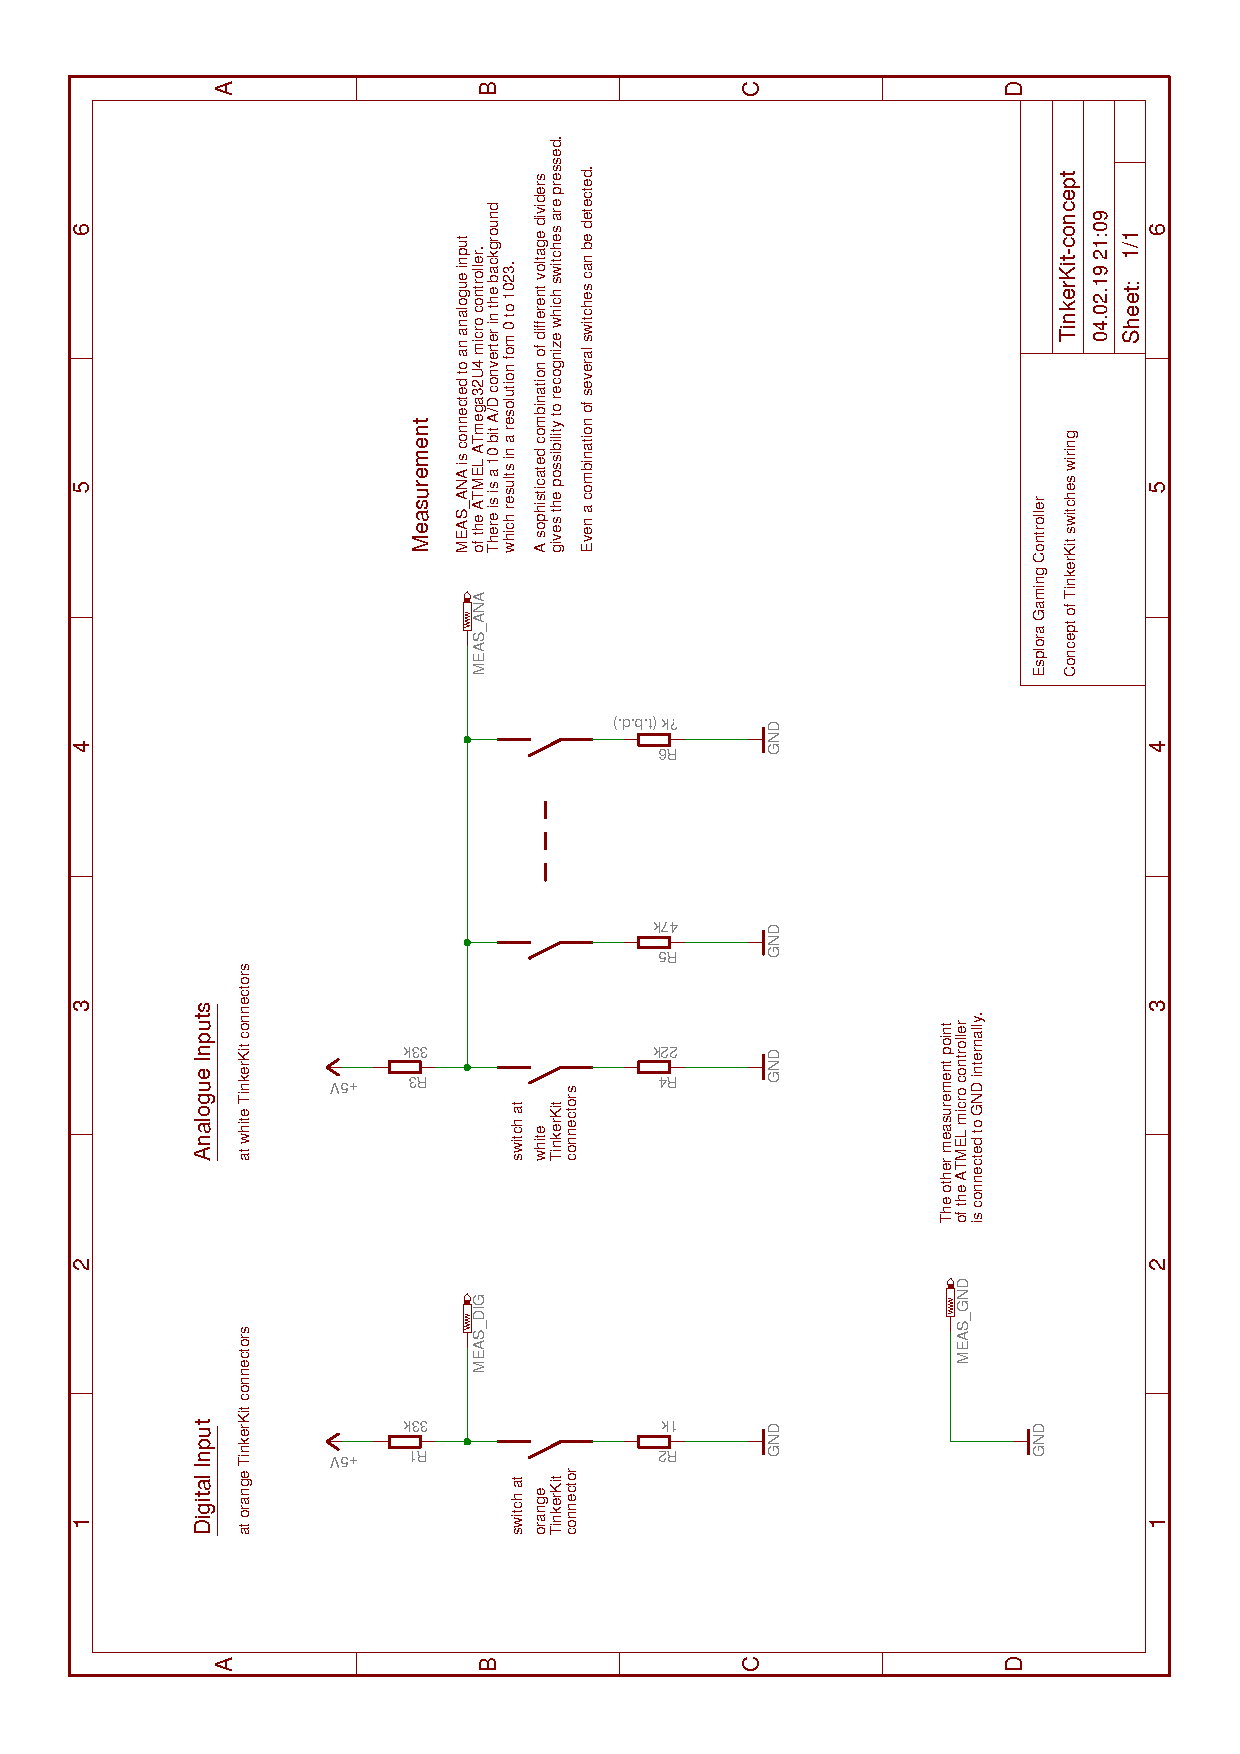
\includepdf[pages=-, portrait, scale=1.0, addtotoc={1,section,0,Konzept,Konzept} ]{./pics/eagle/TinkerKit-concept.pdf}
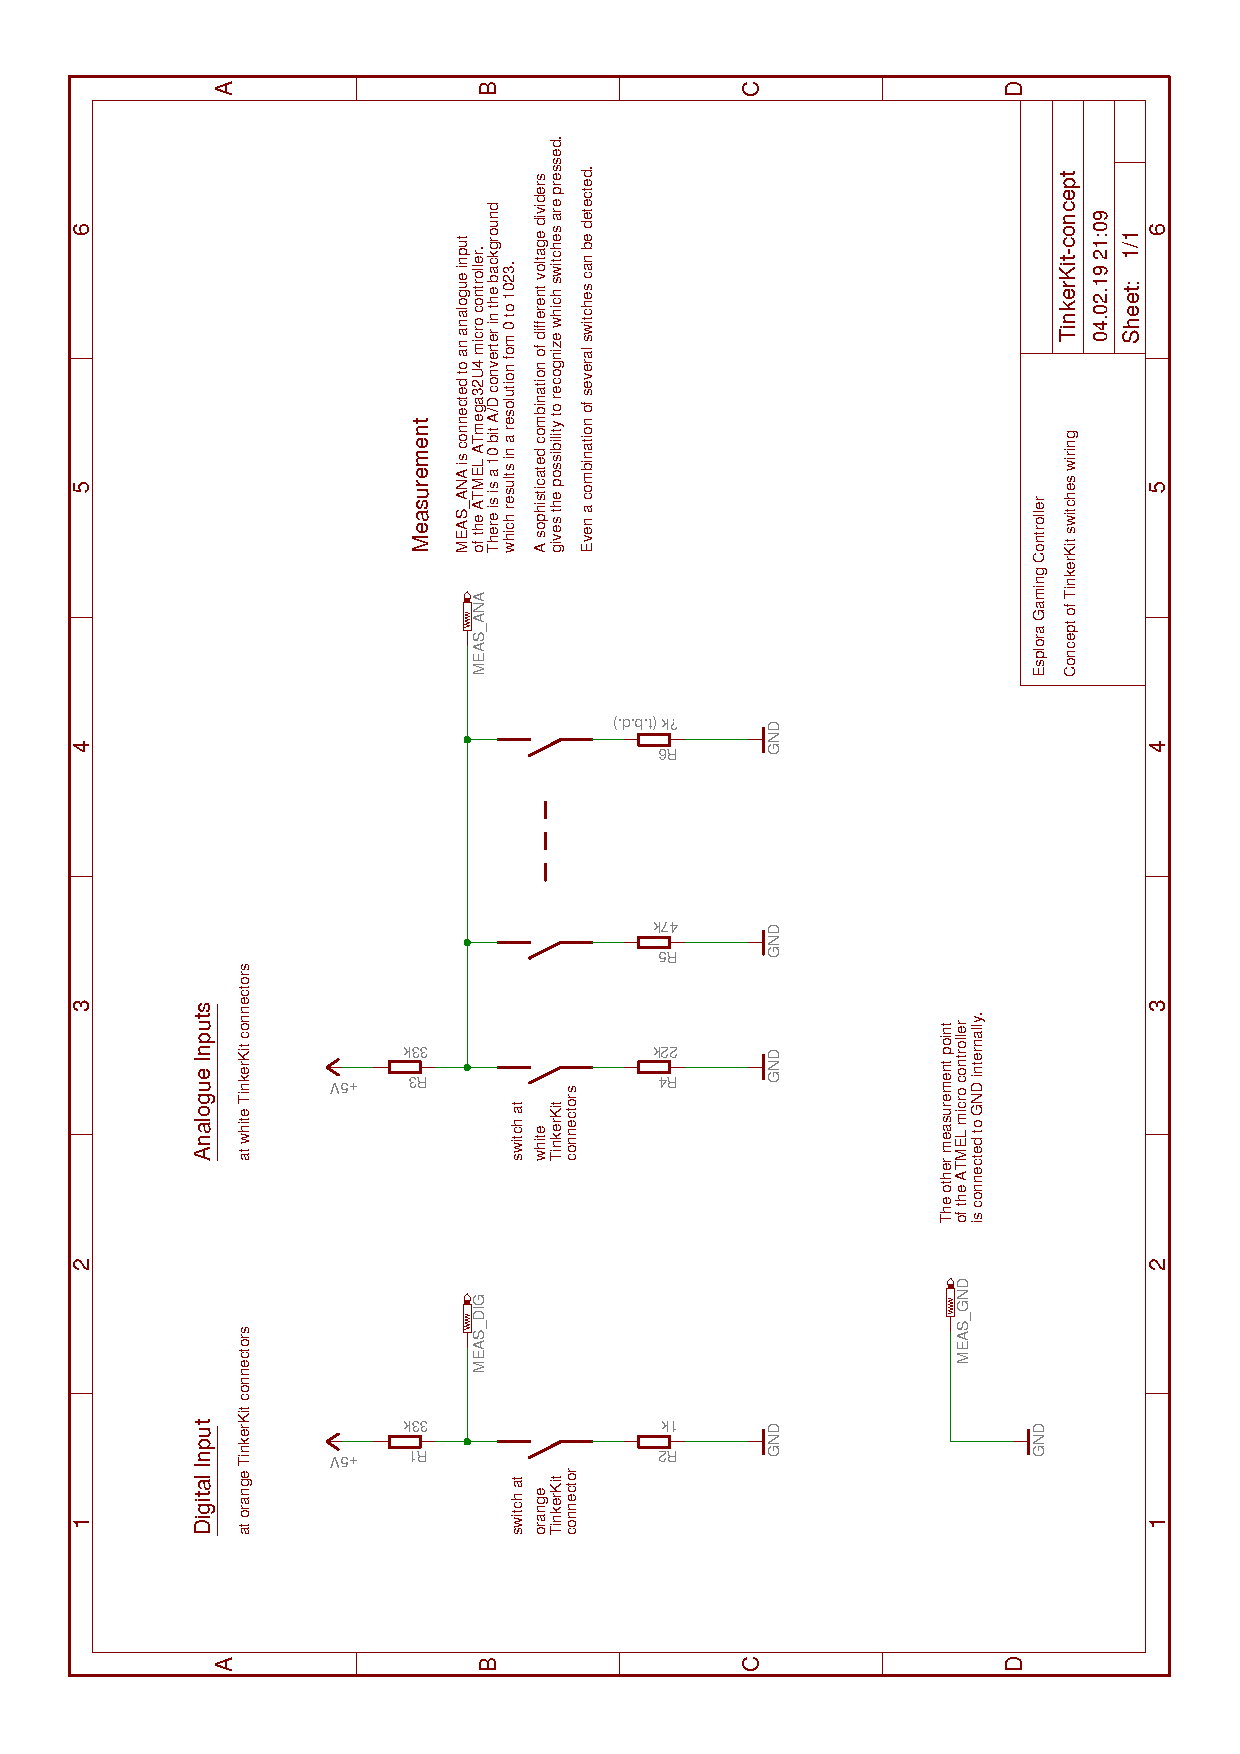
\includepdf[pages=-, , scale=1.0, addtotoc={1,section,0,Konzept,Konzept} ]{./pics/eagle/TinkerKit-concept.pdf}

%---------------------------------------------------------------
%  schematics
%---------------------------------------------------------------
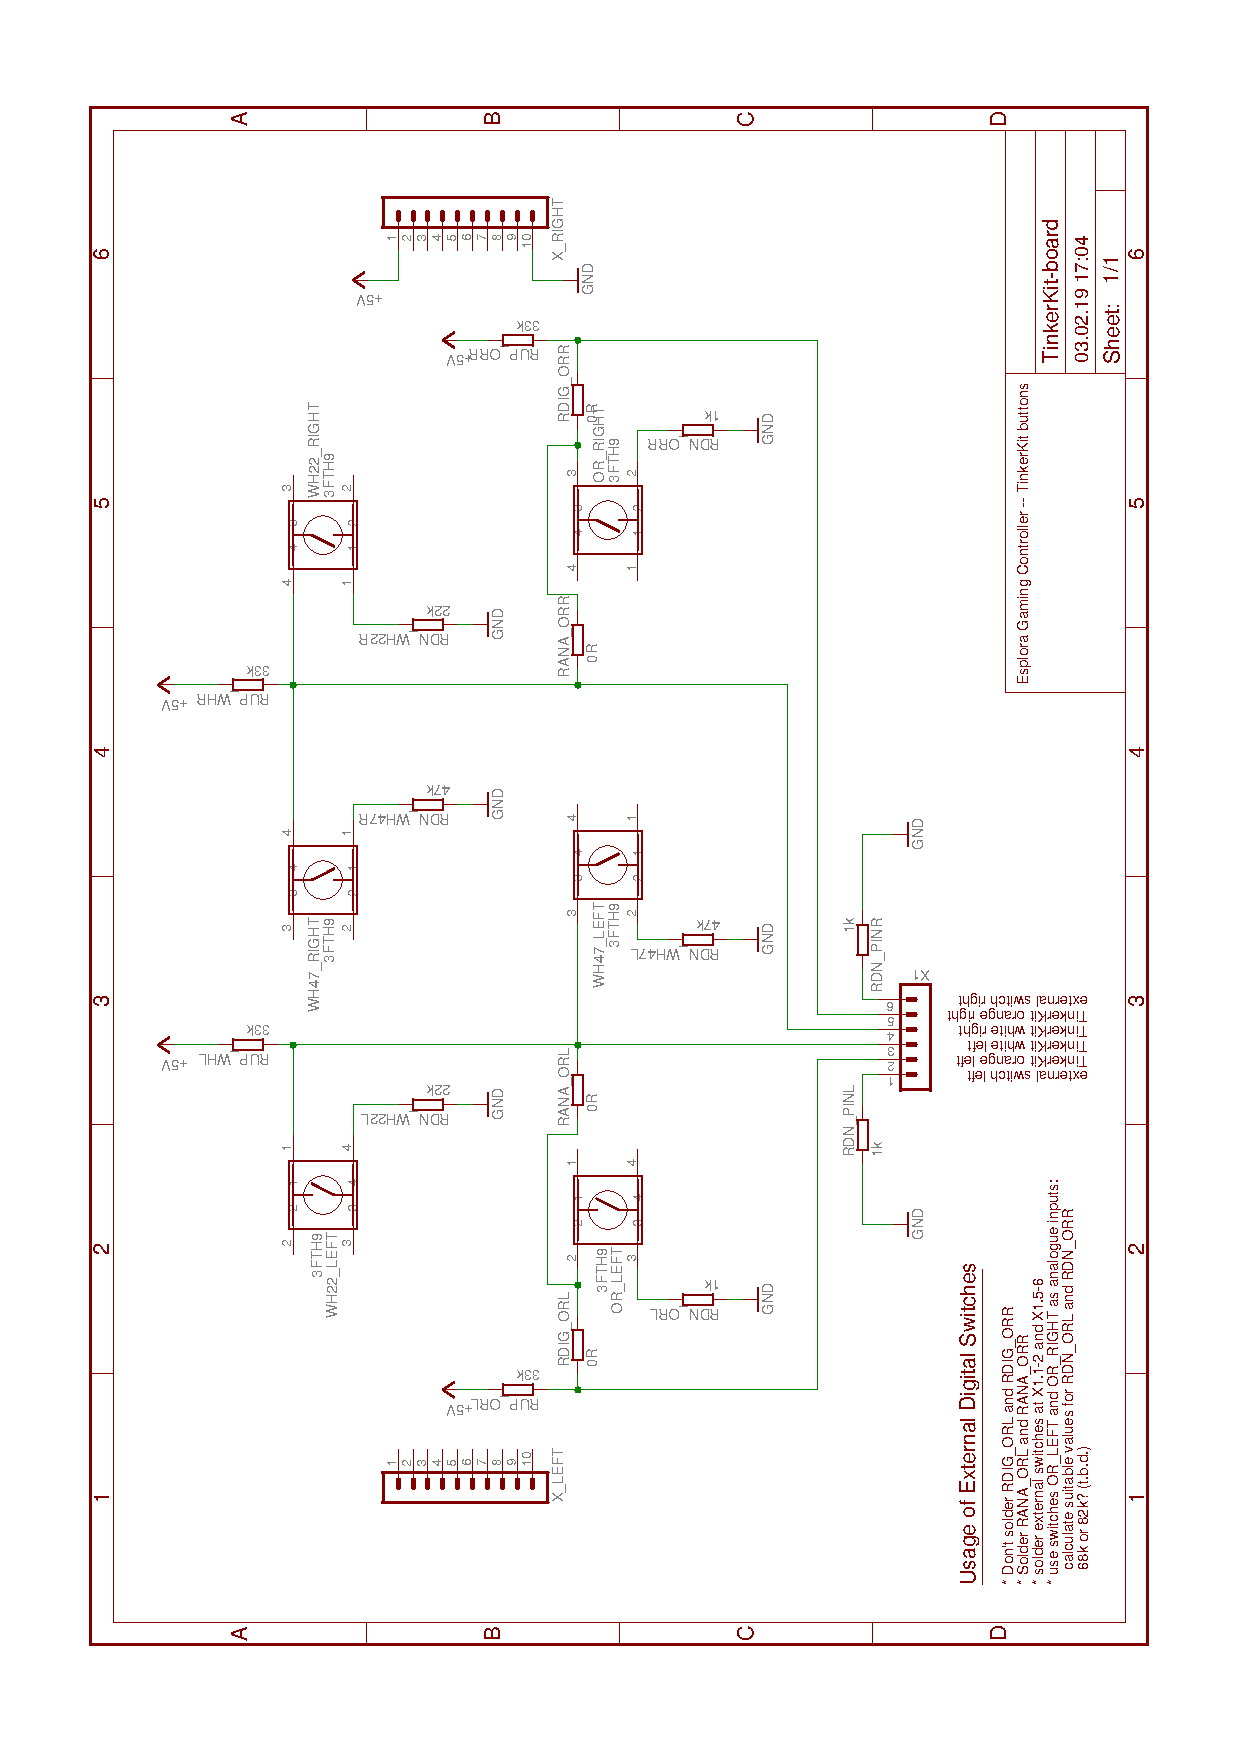
\includepdf[pages=-, , scale=1.0, addtotoc={1,section,0,Zusatzplatine Schaltplan,Zusatzplatine Schaltplan} ]{./pics/eagle/TinkerKit-board_SCH.pdf}

%---------------------------------------------------------------
%  PCB
%---------------------------------------------------------------
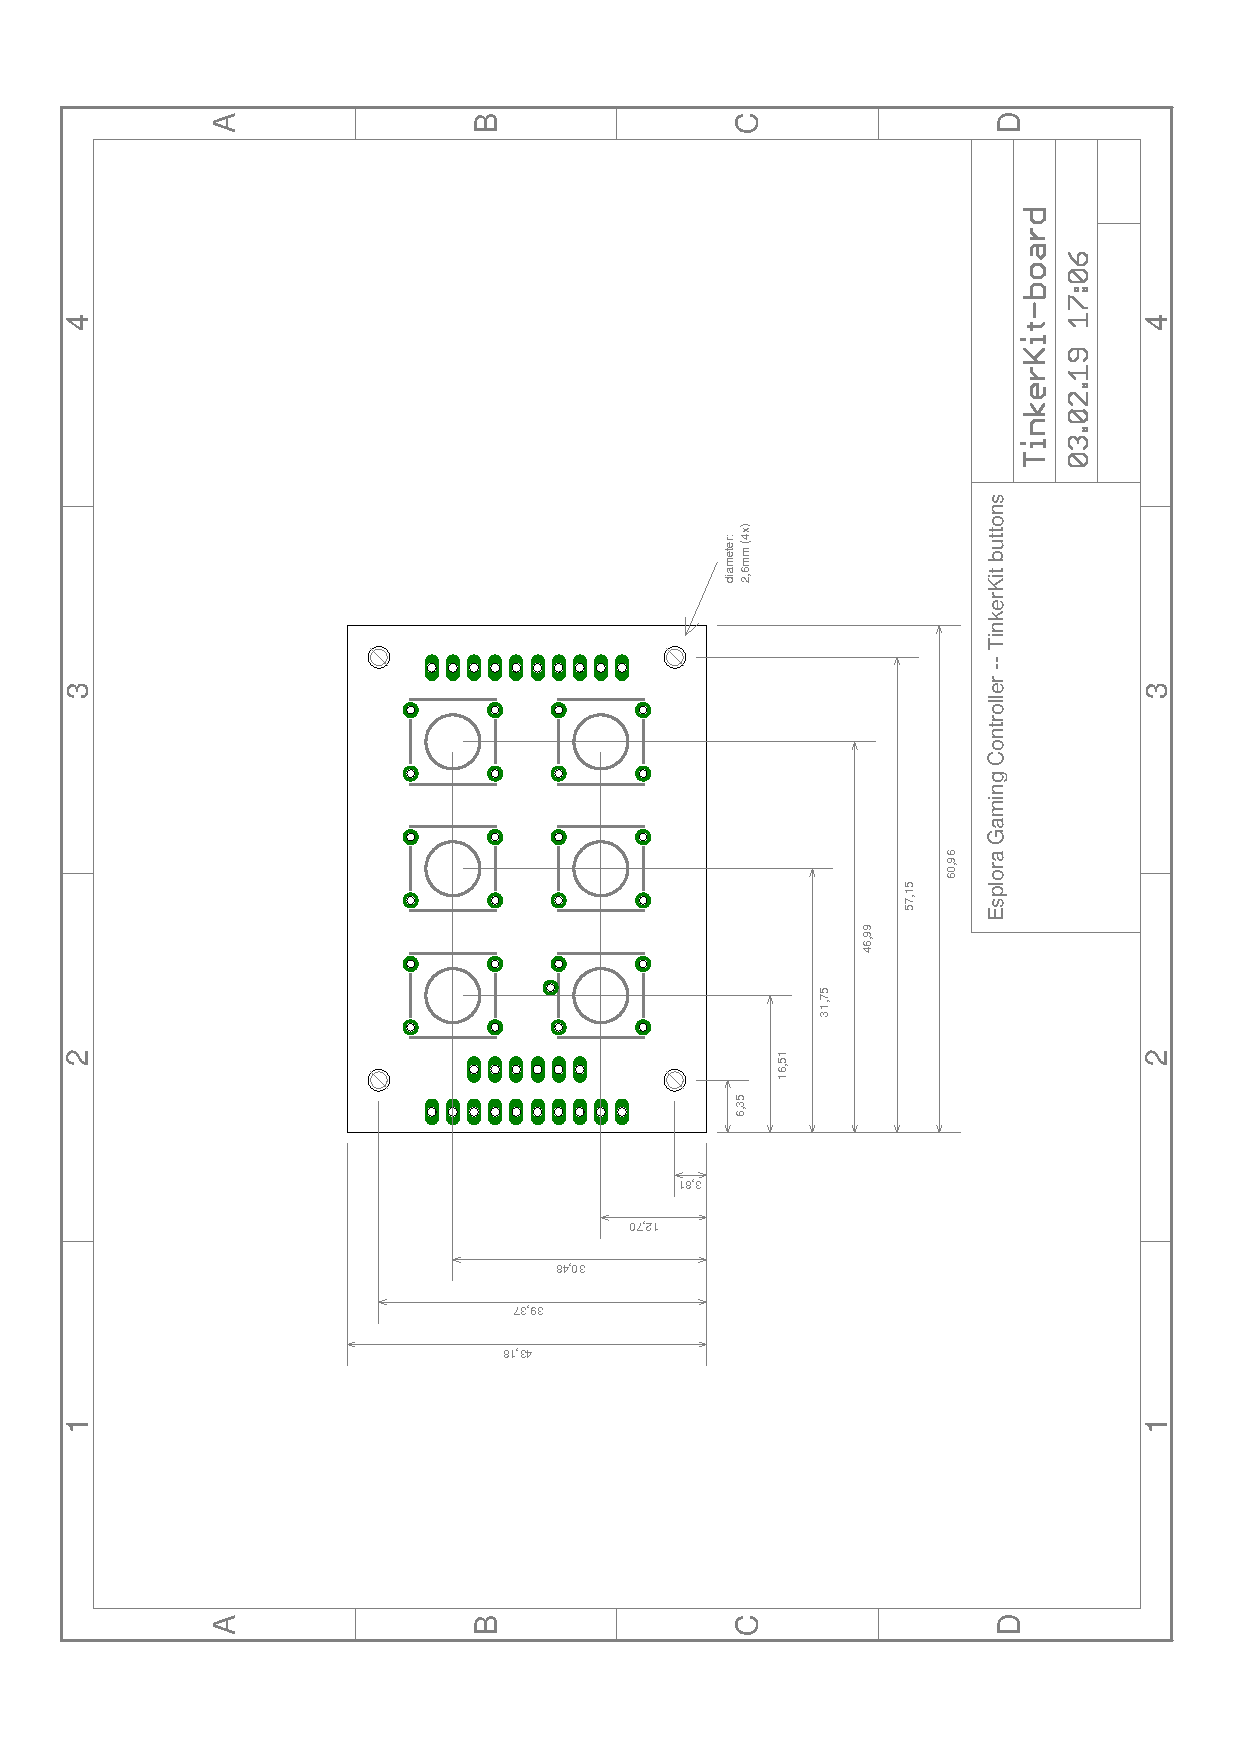
\includepdf[pages=-, , scale=1.0, addtotoc={1,section,0,Zusatzplatine Abmessungen,Zusatzplatine Abmessungen} ]{./pics/eagle/TinkerKit-board_MEAS.pdf}
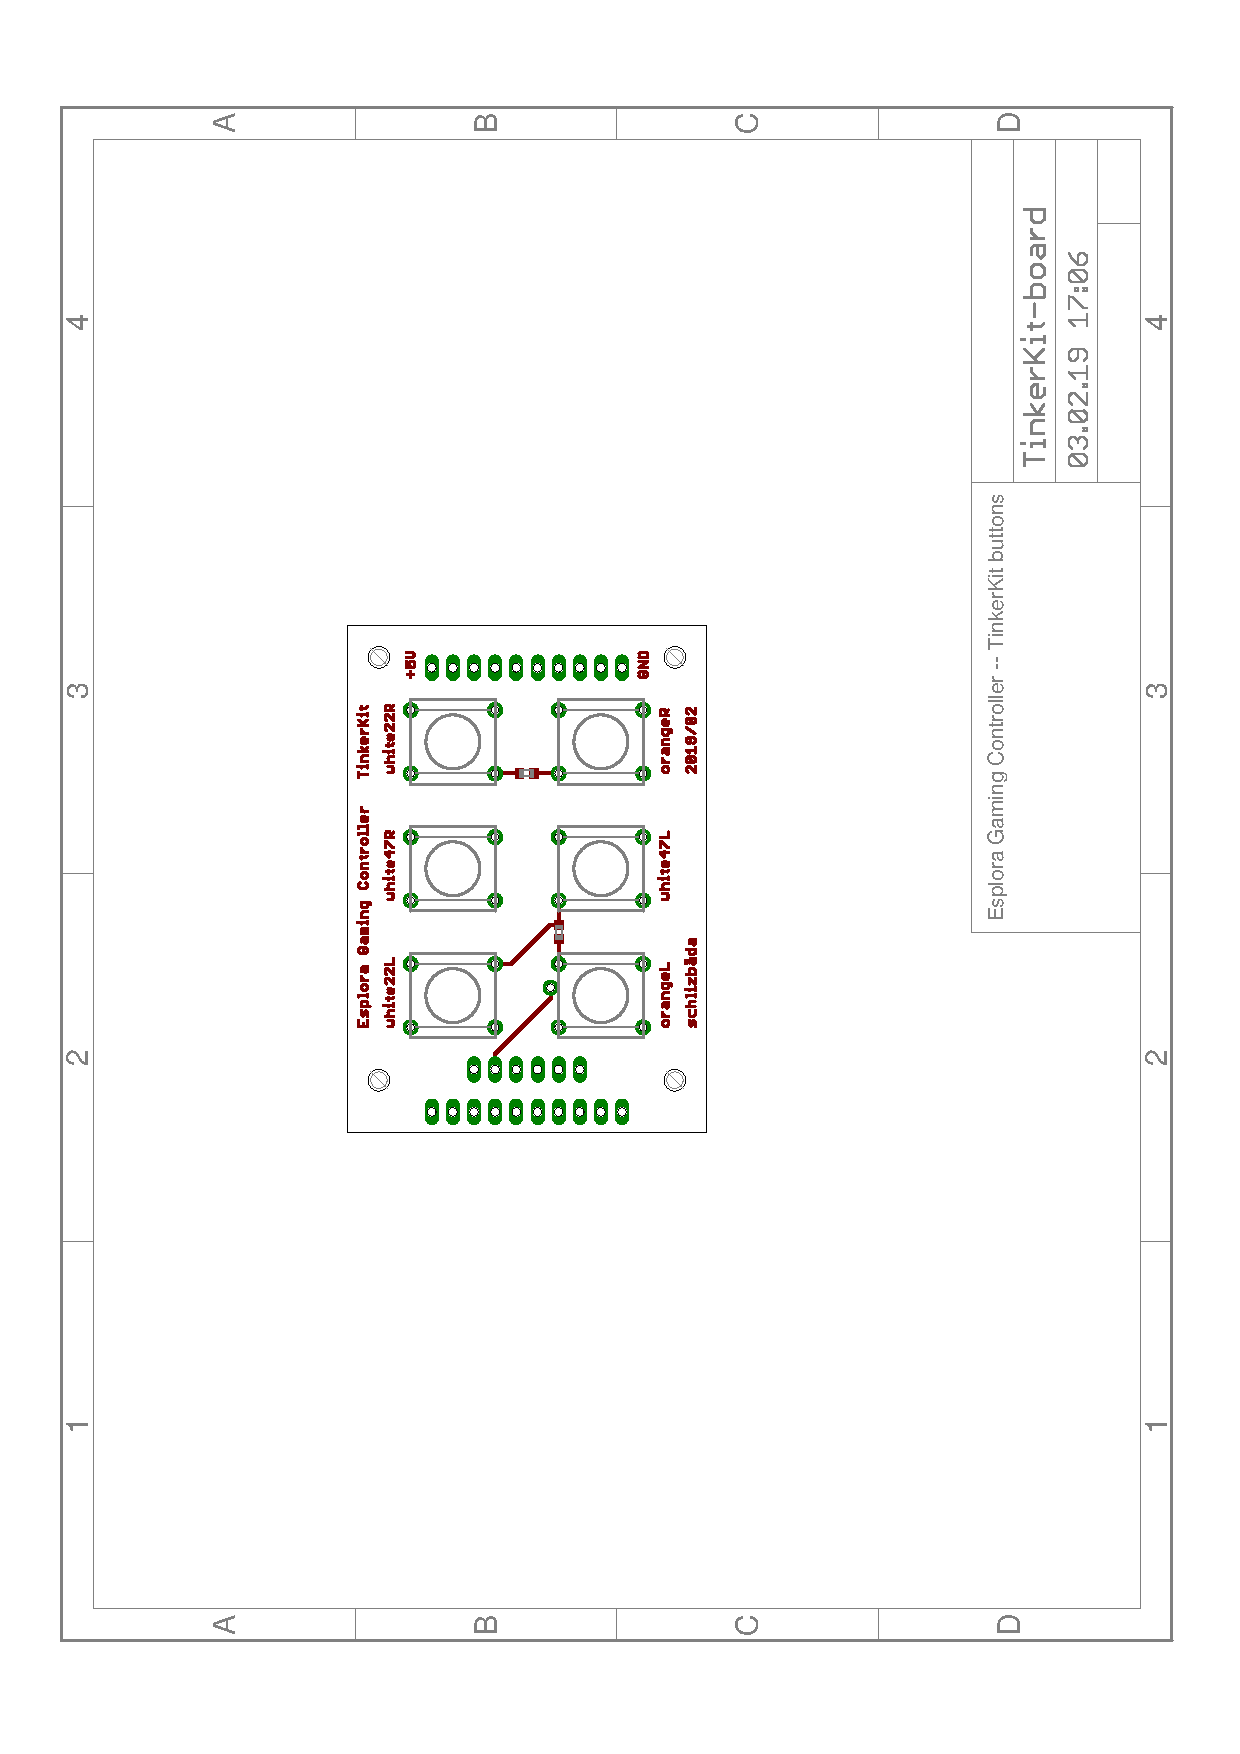
\includepdf[pages=-, , scale=1.0, addtotoc={1,section,0,Zusatzplatine Oberseite,Zusatzplatine Oberseite} ]{./pics/eagle/TinkerKit-board_TOP.pdf}
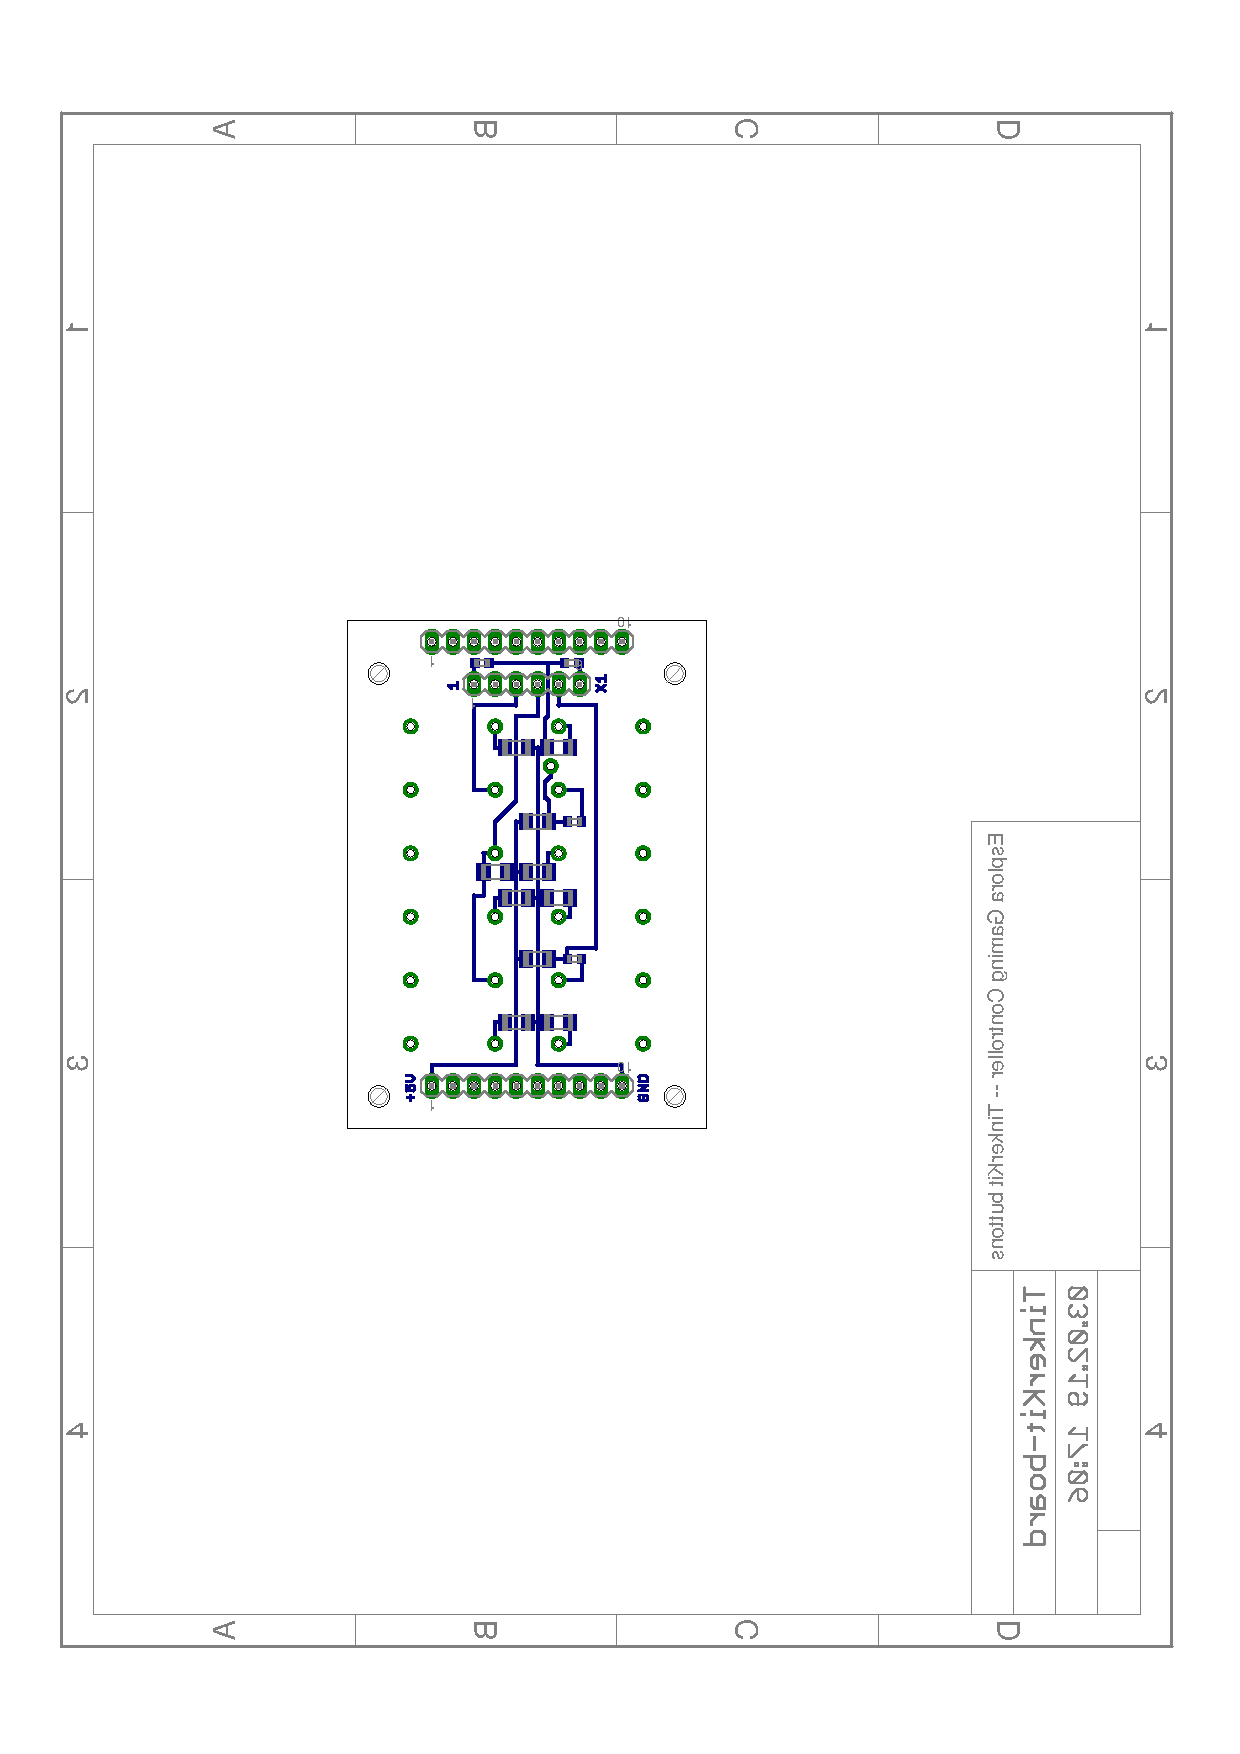
\includepdf[pages=-, , scale=1.0, addtotoc={1,section,0,Zusatzplatine Unterseite,Zusatzplatine Unterseite} ]{./pics/eagle/TinkerKit-board_BOT.pdf}

%%---------------------------------------------------------------
%%  parts
%%---------------------------------------------------------------
%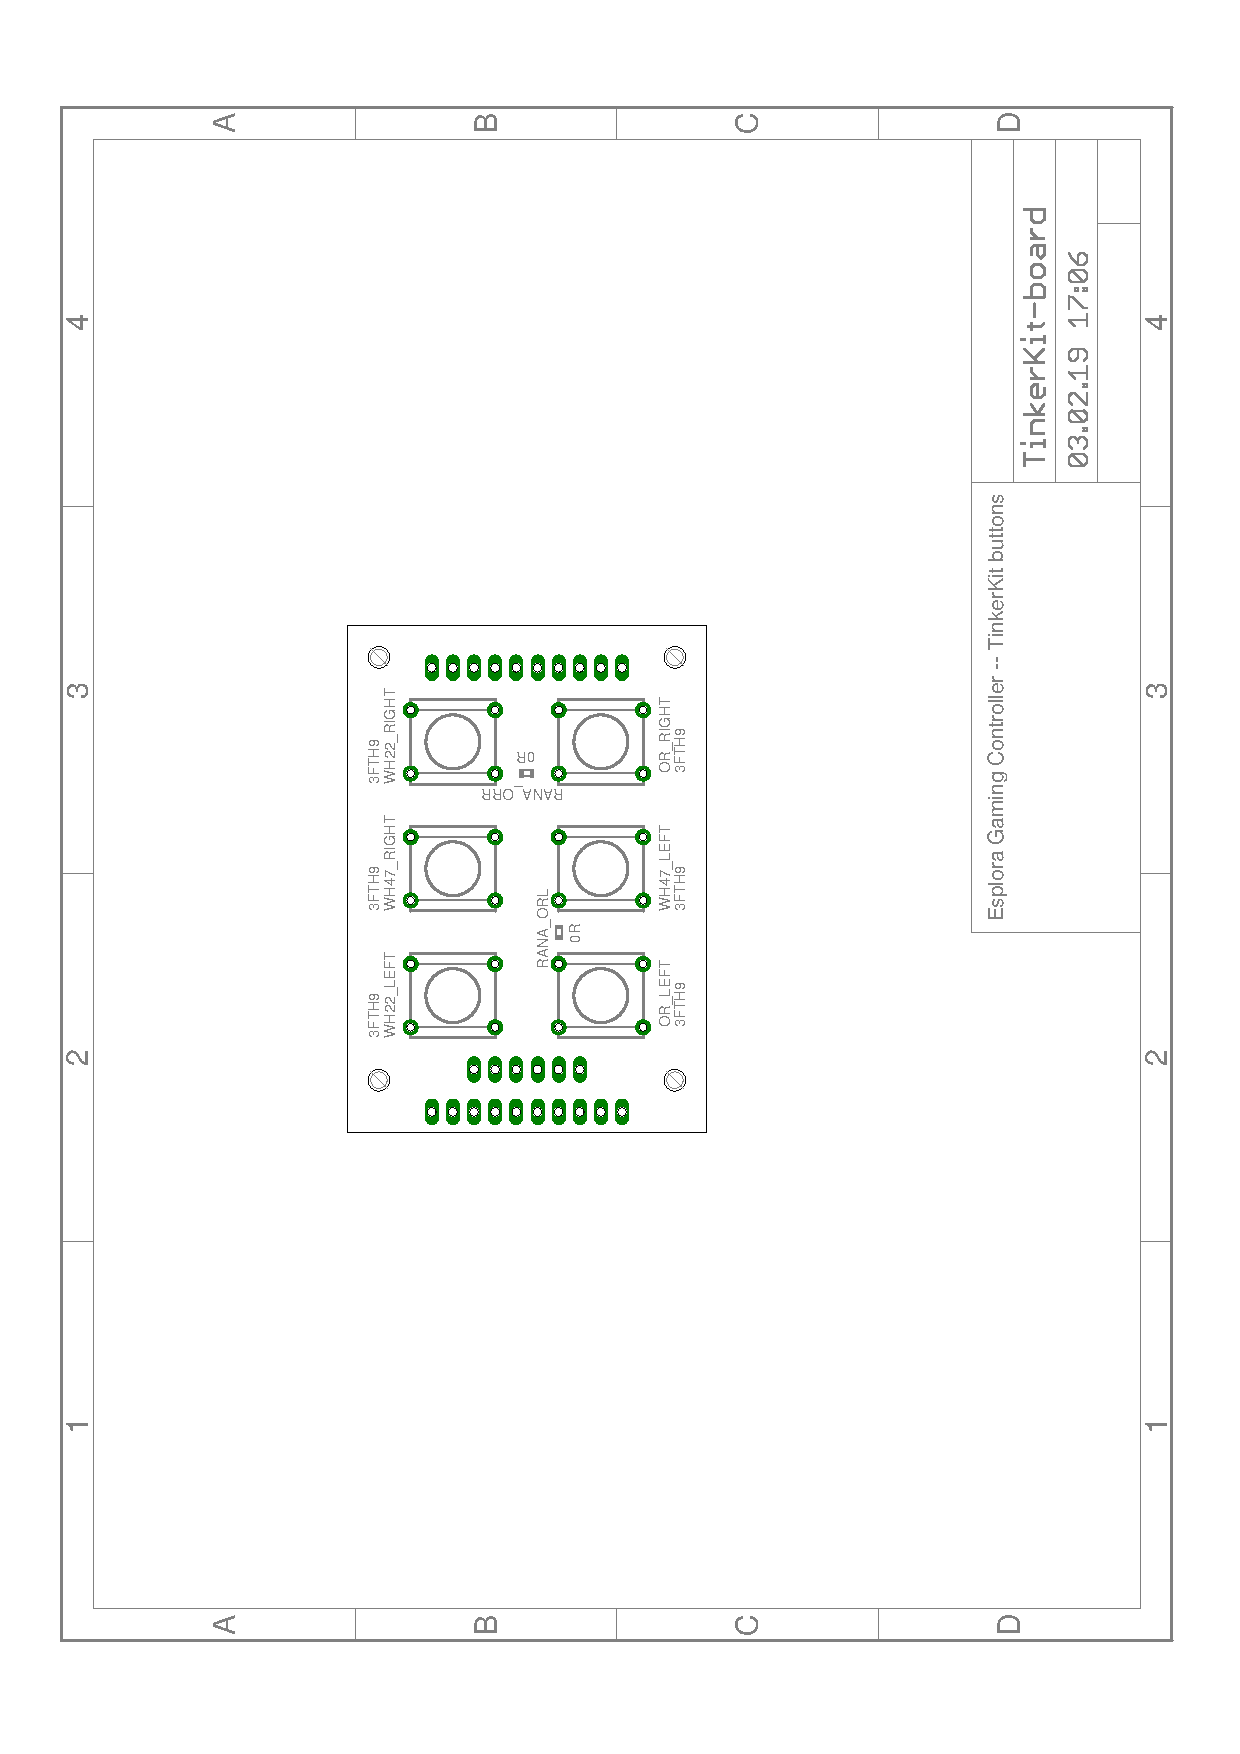
\includepdf[pages=-, , scale=1.0, addtotoc={1,section,0,Leiterplatte,Leiterplatte} ]{./pics/eagle/TinkerKit-board_TOPparts.pdf}
%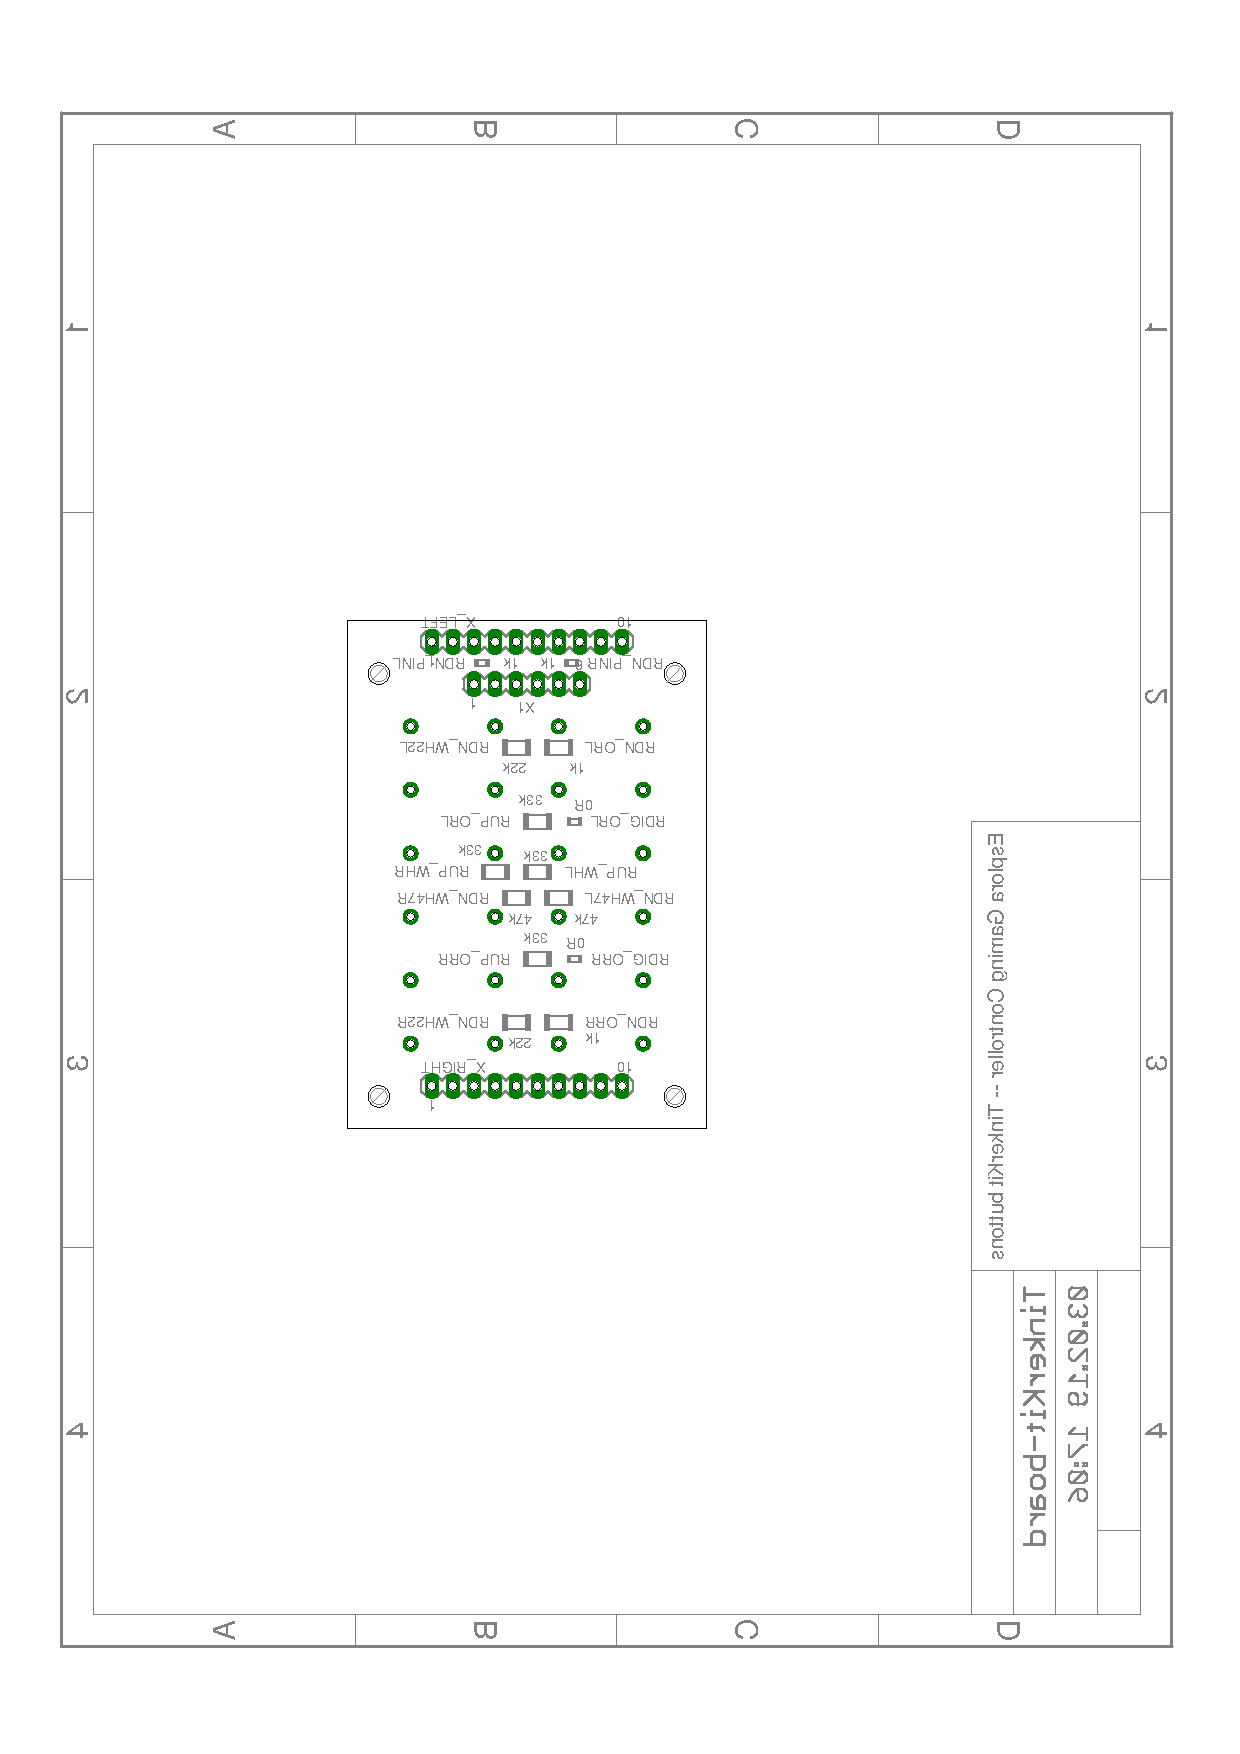
\includepdf[pages=-, , scale=1.0, addtotoc={1,section,0,Leiterplatte,Leiterplatte} ]{./pics/eagle/TinkerKit-board_BOTparts.pdf}
